\section{Исследовательский раздел}

\subsection{Примеры работы}

Фрагмент логов, собранных в /var/log/syslog, приведен на рисунке \ref{logs}.

\begin{figure}[H]
	\centering{
		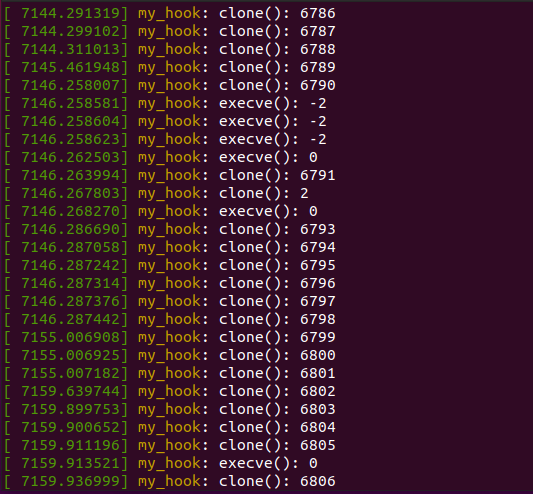
\includegraphics[width=0.8\textwidth]{img/logs.png}
		\caption{Фрагмент /var/log/syslog}
		\label{logs}}
\end{figure}

Результат визуализации собранных данных о системных вызовах с использованием Grafana представлен на рисунках \ref{graf1} и \ref{graf2}.

На первом графике отображены данные за последние 30 минут, сбор метрик проводился каждые 5 минут, а на втором -- за последние 5 минут, сбор метрик проводился каждую минуту. При наведении на график можно увидеть, сколько раз была вызвана каждая функция за последние 10 минут.

\pagebreak

Зеленый график отображает количество вызовов execve(), желтый -- clone().

\begin{figure}[H]
	\centering{
		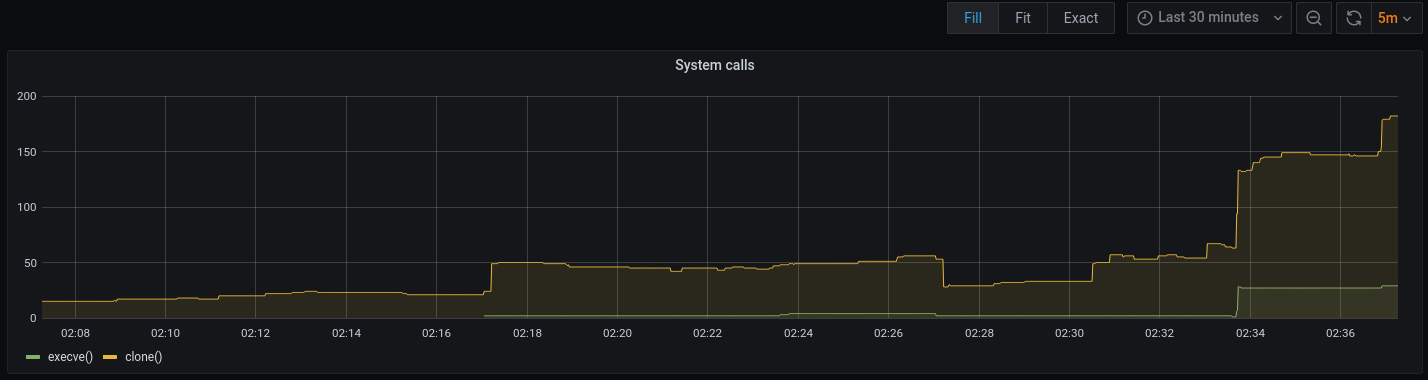
\includegraphics[width=1\textwidth]{img/graf1.png}
		\caption{Вызовы clone() и execve(). Пример 1}
		\label{graf1}}
\end{figure}

\begin{figure}[H]
	\centering{
		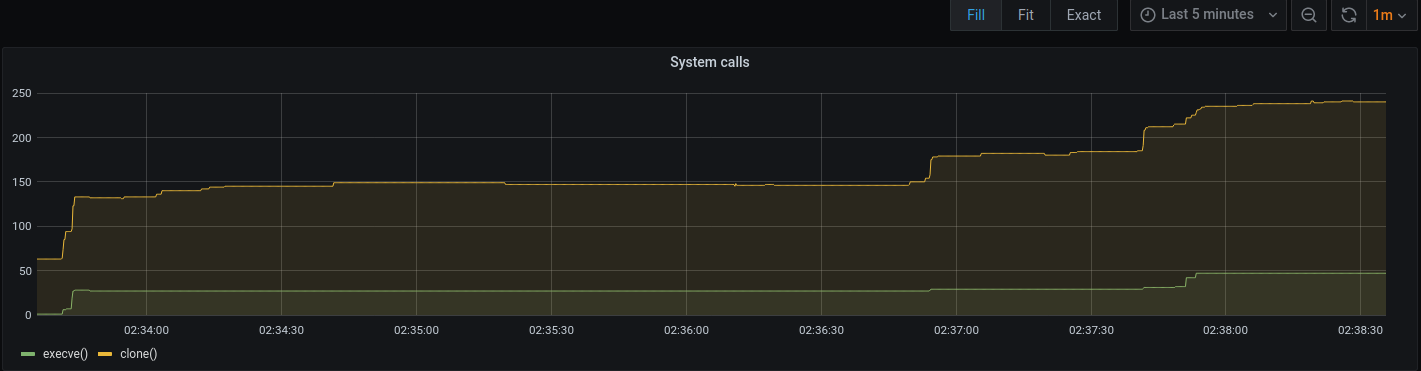
\includegraphics[width=1\textwidth]{img/graf2.png}
		\caption{Вызовы clone() и execve(). Пример 2}
		\label{graf2}}
\end{figure}

\pagebreak